\documentclass{article}
\usepackage{graphicx}
\usepackage{epstopdf}
\usepackage{natbib}
\usepackage{multirow}
\usepackage{amsmath}
\usepackage[dvipsnames]{xcolor}
\usepackage{hyperref}
\usepackage{float} % Needed to force figure dump in specific location. Use [H] option.
\usepackage[left=1in, right=1in, top=1in, bottom=1in]{geometry}
\usepackage{titlesec}
\usepackage[percent]{overpic}
\usepackage{contour}
\usepackage{array}

\newcommand{\genDisc}[1]{\medskip \hrule \vspace{0.25cm}
               {\itshape {\color{violet}{#1}\color{black}} }}
               
\newcommand{\pointRaised}[2]{\medskip \hrule \vspace{0.25cm}
               {\itshape {\bfseries \color{violet}{#1}}: \color{violet}{#2}\color{black}}}
               
\newcommand{\pointRaisedNoRef}[1]{\medskip \hrule \vspace{0.25cm}
               {\itshape {\color{violet}{#1}\color{black}} }}

\newcommand{\reply}{\vspace{0.25cm} \textbf{Reply}:\ }

\newcommand{\zeply}[1]{\vspace{0.25cm} \color{red}\textbf{Reply}:\ {#1}\color{black}}

\newcommand{\todo}[1]{\textcolor{red}{#1}}

\newcommand{\degree}{$^{\circ}$}

\renewcommand{\thefigure}{R\arabic{figure}}
\renewcommand{\thetable}{R\arabic{table}}   

\begin{document}

\title{Author Response to Reviewer \#1 of egusphere-2023-3094, `Algorithmically Detected Rain-on-Snow Flood Events in Different Climate Datasets: A Case Study of the Susquehanna River Basin'}
\author{Colin M. Zarzycki, Benjamin D. Ascher, Alan M. Rhoades, and Rachel R. McCrary}
\date{}

\maketitle
\pagenumbering{gobble}

Specific responses regarding Reviewer \#1's comments are contained in the text that follows. We have highlighted in {\color{Orange}areas in orange} (chosen for color blindness) where we have further refined the manuscript in response to these comments.

\subsection*{Response to Reviewer \#1}

\genDisc{This study makes a useful contribution to studying rain-on-events (at ephemeral snowpacks) by developing and evaluating an algorithm that can detect basin-scale rain-on-snow events using gridded climate data. The method searches for periods of concurrent (area-averaged) precipitation, surface runoff, and snowmelt exceeding pre-defined values. Application of this to Susquehanna River Basin (SRB) indicates that (using dataset-specific thresholds) the method seems to work appropriately. The method also highlights there can be large differences in RoS event magnitude and frequency caused by differences in the various driving factors. 

In principle, this paper could be published, as the developments seem useful, and are logically shown. However, at the same time, the sort of ad-hoc presentation of a single basin results makes it unclear how useful the methods are, and how it’s usefulness varies between scales and settings. This would make the paper more useful and thereby a better fit for this journal.}

\reply{Thank you for agreeing to, and taking the time to, review this work. We have considered the suggestions below and believe addressing them has improved the manuscript.}

\genDisc{It would be useful if a clearer workflow is presented. This helps other people to better understand and potentially adopt the approach}

\reply{
Thank you for the suggestion. We had added some text to better describe the methodology, but the biggest improvement is the addition of a visual schematic that highlights the steps required to take daily, gridded climate data and produce an RoS event climatology as we have done in this paper. We add the below text and figure to the manuscript to better describe the RoS algorithm.

{\color{Orange}
A sample RoS event detection is shown in Fig. 1c.
The smoothed basin-averaged daily time series of PRECIP, ROF, and dSWE are shown from top-to-bottom in dark green, blue, and red respectively (the thinner line represents the raw, unsmoothed time series).
The various thresholds ($t_{\textrm{PRECIP}}$, $t_{\textrm{ROF}}$, and $t_{\textrm{dSWE}}$) are shown as dashed horizontal lines. The area where the metric exceeds the relevant $t$ (i.e., days that the variable's RoS criterion is satisfied) is shaded for each time series.
The vertical black lines denote the start and end of the event, defined by the first and last times when all three quantities exceed their defined threshold $t$.
Gray shading represents contiguous days where all three criteria are satisfied, thus defining a RoS event. Here, an event from January 17th to January 25th, 1996 was added to the record.
}

\begin{figure}[H]
\centering
\noindent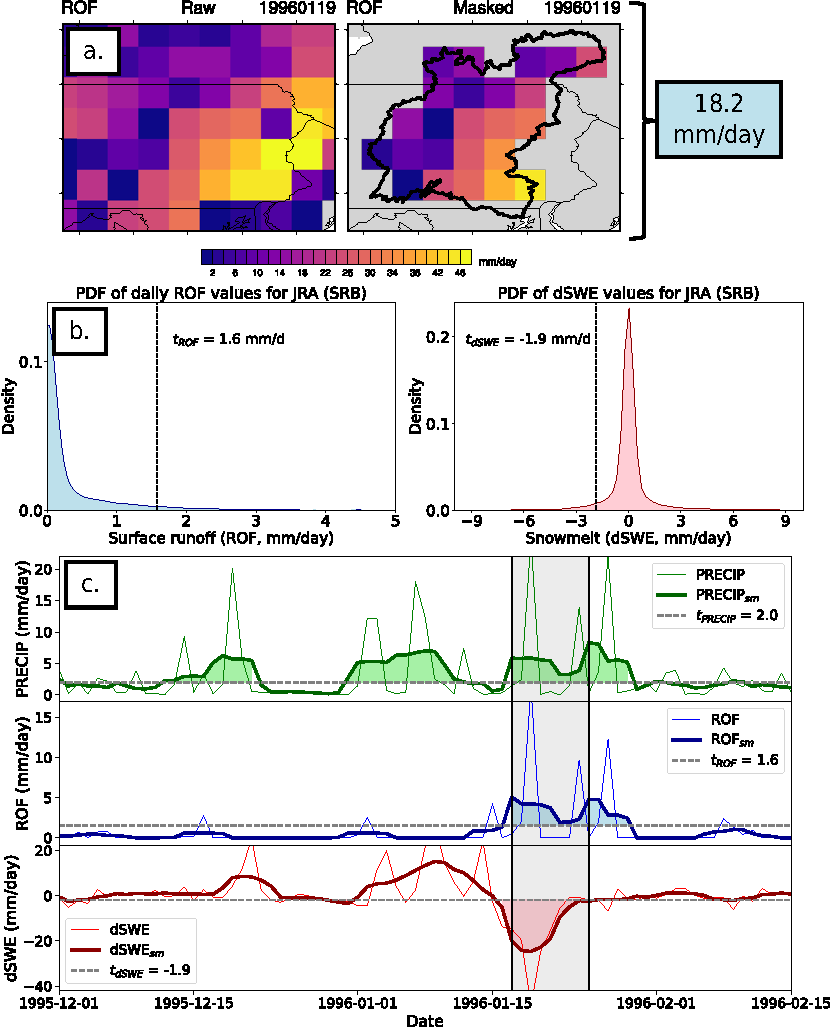
\includegraphics[width=0.65\textwidth]{figs/cropped/schematic.pdf}
\caption{{\color{Orange}Schematic demonstrating how RoS events are defined in this work. (a.) Gridded daily-average data is first masked to only retain data within a defined shapefile (here the SRB) and then area-averaged to produce a single value on that day for the area. (b.) Exceedance thresholds $t$ can be computed from these daily values by using a specified percentile (e.g., 95\%) of the distribution of the entire dataset. (c.) Finally, RoS events are defined as contiguous days where the basin-averaged time series of ROF, dSWE, and PRECIP all exceed their thresholds $t_{\textrm{ROF}}$, $t_{\textrm{dSWE}}$, and $t_{\textrm{PRECIP}}$, respectively. In the bottom plots, the darker lines represent the smoothed timeseries while the thinner lines denote the raw daily data. Shaded areas indicate periods when the given variable's time series is above its relevant threshold $t$ (denoted as a horizontal dashed line).}}
\label{fig:schematic}
\end{figure}
}

\genDisc{The method is applied to one basin. This is OK, but also a bit a thin basis for introducing a method. Across what range of areas is your method likely applicable?

The comparison of climate data for a single basin (section 3.1) is useful, but it would be a lot more useful to systematically test how these things vary? (i.e. beyond this specific basin).}

\reply{This is similar to the suggestion from Reviewer \#2 about generalizability. While a global (or even large-scale regional) evaluation of how well the technique transfers to other basins is beyond the scope of this work, we add a new section to the manuscript entitled {\color{Orange}`\textbf{Generalizability to other basins}.'} We have reproduced this new text in the Appendix of this response.

In this section we test the RELATIVE configuration of the algorithm in two additional basins in the western United States: the Willamette River Basin (WRB) in Oregon and southern Washington and the Sacramento River Basin (SacRB), covering parts of Northern California and Southern Oregon. We evaluate two water years where notable rain-on-snow events occurred -- a flood in the WRB in February 1996 and one in the SacRB at the end of December 1996 into January 1997. We find that the algorithm detects these RoS events without additional modification/tuning, which we take as a positive sign that the framework could be extended to other basins. In addition to a cursory comparison of the four datasets, we also note that there are potential ways to further improve this framework by using larger hydrologic units, modifying the regions in which data is averaged over, etc.}

\genDisc{The timescale over which RoS are relevant will be very dependent on the spatial scale of the watershed. For example, headwater catchments may need timescales of hours whereas for large basins it may be multiple days. Can this be discussed?}

\reply{This is a good point. We have added additional text in the discussion section that notes that the findings here are tied to both the spatial and temporal scales of the hydrologic processes in addition to the forcing/coupling frequency.

{\color{Orange}``We also show that even though a dataset is provided at much coarser spatial resolutions than is desired (e.g., JRA and E3SM), model-derived datasets that are more frequently coupled and/or constrained at shorter timescales (e.g., reanalysis products and nudged ESMs) may produce more accurate land-atmosphere interactions and better representation of decision-relevant hydrometeorological extremes, particularly at basin (and larger) spatial scales. However, these products will likely suffer in the spatial representation of hydrometeorology in regions of high heterogeneity. The spatial resolution is also tightly linked to land surface flood processes within the basin. Higher resolution may better resolve headwater catchments and smaller geometries whereas coarser datasets may only be skillful at larger scales, even with more accurate forcing. Spatial scales are also connected to hydrologic timescales. Smaller areas respond to increased liquid input more quickly than larger, downstream sections of a basin. Understanding how coupling frequency affects hydrologic climate data, alongside spatial and temporal characteristics, is a complex challenge, but may offer insights into improving dataset credibility''}}

\genDisc{Provide units at all axes go all figures.}

\reply{Thank you for catching that! We have carefully gone through the manuscript and all figures have been updated to better describe units on all axes.}

\appendix
\renewcommand{\thesection}{Appendix \Alph{section}:}
\section{Generalizability to other basins}

\textit{Author note: The below block of code will be a new section in a revised manuscript.}\\

Finally, while we focus on the SRB in this manuscript, it is beneficial to evaluate whether the algorithm can detect other well-known historical RoS events in the US and whether the dataset-to-dataset variability observed in the SRB occurs elsewhere.
As a test of the transferability of the methodology described in Section 2.2, we perform the same analysis using the RELATIVE framework over the Willamette River Basin (WRB) in Oregon and southern Washington and Sacramento River Basin (SacRB), covering parts of Northern California and Southern Oregon in the United States.
A significant RoS flood event occurred over the WRB in 1996 a few weeks following the SRB event discussed above.
From February 5th-9th, 1996, the WRB experienced its most severe flooding in three decades, with parts of the river rising up to 3-6 meters above flood stage, causing eight fatalities, displacing over 30,000 residents, and causing nearly \$500 USD million in damages.
Preceding the floods, subfreezing temperatures and substantial snowpack prevailed at relatively low elevations, but a succession of warmer synoptic systems brought liquid precipitation ranging from 10-25 cm in lowlands to 35-75 cm in mountainous regions over the four-day period.
These conditions led to significant snowmelt, exacerbating the flooding \citep{halpert1997climate,colle2000february}.
The 1997 New Year's flood event in California was the most financially devastating flood in the state's history with damages totaling \$1.6 USD billion, ranked as the second most severe superflood between 1950 and 2010 across the western United States \citep{tarouilly2021western}.
Over half a million individuals were displaced, and 43 out of 58 California counties were declared disaster zones \citep{lott1997}.
Preceding storms in late November and December contributed to elevated soil moisture and a substantial snowpack, setting the stage for extreme flooding exacerbated by heavy precipitation and an intense, warm, atmospheric river event on New Year's Day of 1997 \citep{galewsky2005moist,rhoades2023recreating}.

\begin{figure}[H]
\noindent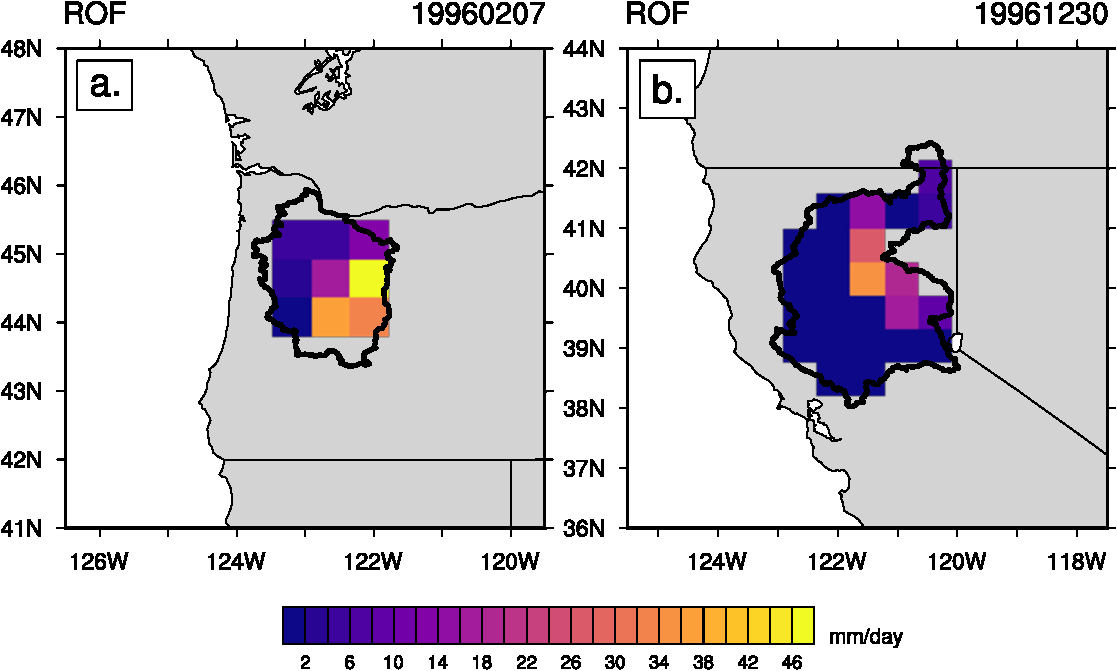
\includegraphics[width=0.7\textwidth]{figs/cropped/other_basins_ROF.pdf}
\caption{Basin shapefile domains for (a.) the Willamette River Basin (WRB) and (b.) the Sacramento River Basin (SacRB). Contoured is the surface runoff field from JRA on (a.) February 7th, 1996, and (b.) December 30th, 1996.}
\label{fig:otherbasins}
\end{figure}

To probe these events, we first acquire shapefiles defining both the WRB and SacRB, shown in Fig. \ref{fig:otherbasins}.
Like with the SRB analysis, all four datasets are masked using these basins.
Daily, basin-averaged mean timeseries are constructed with the 95\% percentiles of ROF and dSWE being computed from these distributions to use as thresholds $t_{\textrm{ROF}}$ and $t_{\textrm{dSWE}}$.
We then seek RoS events by looking for periods of concurrent PRECIP, ROF, and dSWE that all exceed relevant thresholds.

Fig. \ref{fig:ros-wrb} shows the WY96 results over the WRB. The February flood event is clearly evident in the streamflow shading along the top of the panels on the left (black colors indicating 99.9\% streamflow).
Three of the four products indicate a RoS event immediately preceding this streamflow maximum.
All products indicate spikes in PRECIP and ROF over the basin, although E3SM produces less precipitation than the other three, likely owing to its coarser resolution.
JRA has the largest and most rapid snowmelt, with both NLDAS and E3SM also showing reductions in SWE during the event.
L15 shows a small rapid increase, then a decrease in SWE during the event.
This offset is strong enough that the RoS algorithm is not triggered ($t_{\textrm{dSWE}}$ is not satisfied).
While a more detailed evaluation of the meteorology as represented by the data products is beyond the scope of this study, it is possible that some of the mechanisms discussed in Section 3.4 are also relevant in this basin.
The bubble plots on the right side of Fig. \ref{fig:ros-wrb} show a wide diversity as in Fig. 6, although the relative differences are somewhat dissimilar, implying different processes are at play, particularly for the ROF.
As before, L15 has a narrower range of dSWE over the basin (i.e., spread on the horizontal axis) but does contain large values of both precipitation (vertical axis) and runoff (marker size).
The dSWE variability for both E3SM and JRA is larger but the products generally have lower ROF and PRECIP, respectively, than both L15 and NLDAS.

\begin{figure}[H]
\centering
\begin{tabular}{@{}m{0.45\textwidth}@{\hspace{1.5em}}m{0.3\textwidth}@{}}

\begin{overpic}[width=\linewidth]{figs/cropped/L15_WillametteBasin_events.pdf}
\put (11,39.5) {\contour{white}{\large a.}}
\end{overpic}
&
\begin{overpic}[width=\linewidth]{figs/cropped/L15_WillametteBasin_scatplot.pdf}
\put (14,61.0) {\contour{white}{\large b.}}
\end{overpic}
\\
\begin{overpic}[width=\linewidth]{figs/cropped/NLDAS_WillametteBasin_events.pdf}
\put (11,39.5) {\contour{white}{\large c.}}
\end{overpic}
&
\begin{overpic}[width=\linewidth]{figs/cropped/NLDAS_WillametteBasin_scatplot.pdf}
\put (14,61.0) {\contour{white}{\large d.}}
\end{overpic}
\\
\begin{overpic}[width=\linewidth]{figs/cropped/JRA_WillametteBasin_events.pdf}
\put (11,39.5) {\contour{white}{\large e.}}
\end{overpic}
&
\begin{overpic}[width=\linewidth]{figs/cropped/JRA_WillametteBasin_scatplot.pdf}
\put (14,61.0) {\contour{white}{\large f.}}
\end{overpic}
\\
\begin{overpic}[width=\linewidth]{figs/cropped/E3SM_WillametteBasin_events.pdf}
\put (11,39.5) {\contour{white}{\large g.}}
\end{overpic}
&
\begin{overpic}[width=\linewidth]{figs/cropped/E3SM_WillametteBasin_scatplot.pdf}
\put (14,61.0) {\contour{white}{\large h.}}
\end{overpic}
\\
\end{tabular}
\caption{As in Figs. 5 (a., c., e., g.) and 6 (b., d., f., h.), except for the Willamette River Basin (WRB) during WY96. The striped gauge percentiles along the top of the left panels are derived from daily streamflow from USGS gage \#14211720 (Willamette River at Portland, Oregon).}
\label{fig:ros-wrb}
\end{figure}

Figure \ref{fig:ros-sacrb} shows the WY97 results over the SacRB.
Here, all four data products detect a RoS event in the basin in late December/early January.
The timing differs slightly between the datasets, with E3SM (L15) triggering the earliest (latest).
We speculate that this is a function of resolution, where the higher-resolution L15 contains more detailed small-scale processes (e.g., sub-basin melt at higher elevations, time for headwaters to reach the main stem).
Evaluating temporal differences at the daily scale due to model structural characteristics is an interesting target for future work.
All products capture large spikes in PRECIP and subsequent increases in ROF over the basin.
They differ more significantly in terms of dSWE, with JRA (NLDAS) producing the most (least) snowmelt over the basin.
Of note, both JRA and E3SM flag a smaller RoS event later in January while both L15 and NLDAS show increased SWE in the basin.
All products show increases in ROF, however, which coincide with a secondary maximum in the streamflow, highlighting the complexity of how surface hydrology evolves in models even if the relevant metrics (e.g., runoff) are similar.
The bubble plots on the right of Fig. \ref{fig:ros-sacrb} indicate similar behavior to Fig. \ref{fig:ros-wrb}, which is likely a function of snow processes in the SacRB being more similar to the WRB than the SRB.

\begin{figure}[H]
\centering
\begin{tabular}{@{}m{0.45\textwidth}@{\hspace{1.5em}}m{0.3\textwidth}@{}}
\begin{overpic}[width=\linewidth]{figs/cropped/L15_SacRB_USGS1802_events.pdf}
\put (11,39.5) {\contour{white}{\large a.}}
\end{overpic}
&
\begin{overpic}[width=\linewidth]{figs/cropped/L15_SacRB_USGS1802_scatplot.pdf}
\put (14,61.0) {\contour{white}{\large b.}}
\end{overpic}
\\
\begin{overpic}[width=\linewidth]{figs/cropped/NLDAS_SacRB_USGS1802_events.pdf}
\put (11,39.5) {\contour{white}{\large c.}}
\end{overpic}
&
\begin{overpic}[width=\linewidth]{figs/cropped/NLDAS_SacRB_USGS1802_scatplot.pdf}
\put (14,61.0) {\contour{white}{\large d.}}
\end{overpic}
\\
\begin{overpic}[width=\linewidth]{figs/cropped/JRA_SacRB_USGS1802_events.pdf}
\put (11,39.5) {\contour{white}{\large e.}}
\end{overpic}
&
\begin{overpic}[width=\linewidth]{figs/cropped/JRA_SacRB_USGS1802_scatplot.pdf}
\put (14,61.0) {\contour{white}{\large f.}}
\end{overpic}
\\
\begin{overpic}[width=\linewidth]{figs/cropped/E3SM_SacRB_USGS1802_events.pdf}
\put (11,39.5) {\contour{white}{\large g.}}
\end{overpic}
&
\begin{overpic}[width=\linewidth]{figs/cropped/E3SM_SacRB_USGS1802_scatplot.pdf}
\put (14,61.0) {\contour{white}{\large h.}}
\end{overpic}
\\
\end{tabular}
\caption{As in Figs. 5 (a., c., e., g.) and 6 (b., d., f., h.), except for the Sacramento River Basin (SacRB) during WY97. The striped gauge percentiles along the top of the left panels are derived from daily streamflow from USGS gage \#14211720 (Sacramento River at Verona, California).}
\label{fig:ros-sacrb}
\end{figure}

While this should only be considered a cursory investigation, it provides additional data points that the methodology can be applicable to other basins susceptible to RoS flooding.
Of note, both the WRB and SacRB contain higher and steeper orography than the SRB, implying that the algorithm can credibly detect RoS events in different basin geometries.
However, we stress a few caveats. More rigorous evaluation would be required by regional hydrologists to ensure results in other basins are hydrologically fit-for-purpose.
Further, we also acknowledge that RoS over high mountain ridges can feed into rises in streamflow in different basins (e.g., the Sierra Nevada mountains in California contribute to multiple watersheds).
Applying shapefiles containing larger hydrologic units or other spatial coverage may improve results in these regions and provide a better understanding of model variability and how land surface processes are represented in climate data.


\bibliographystyle{abbrvnat}
\bibliography{refs-ros-metrics.bib} 

\end{document}